\documentclass[aspectratio=169,12pt]{beamer}
\usepackage[utf8]{inputenc}
\usepackage{amsmath, amssymb}
\usepackage{booktabs}
\usepackage{colortbl}
\usepackage{hyperref}
\usepackage{makecell}
\usepackage{ragged2e}
\usepackage{bytefield}
\usepackage{tikz}
\usetikzlibrary{arrows.meta, positioning, shapes.geometric, calc, tikzmark, shapes.misc, fit, backgrounds, decorations.pathreplacing}
\usepackage{tcolorbox}
\usepackage{listings}
\usepackage{xcolor}
\usetheme{Madrid}

\title{Cache Memory II}
\author{Computer Architecture 2340267}
\date{2025, Recitation \#4}

% Macro for memory hierarchy diagram
\newcommand{\memoryhierarchy}[1][1]{%
\begin{tikzpicture}[scale=#1]
    % Cache levels (L1 on top)
    \node[draw, fill=white, thick, minimum width=4cm, minimum height=0.6cm, rectangle, font=\small\bfseries] (l3) {L3 Cache};
    \node[draw, fill=white, thick, minimum width=3.5cm, minimum height=0.6cm, rectangle, font=\small\bfseries, above=0.1cm of l3] (l2) {L2 Cache};
    \node[draw, fill=white, thick, minimum width=3cm, minimum height=0.6cm, rectangle, font=\small\bfseries, above=0.1cm of l2] (l1) {L1 Cache};

    % Multi-level cache container - drawn in background layer
    \begin{scope}[on background layer]
        \node[draw, fill=red!30, thick, rectangle, fit=(l1)(l2)(l3), inner sep=0.15cm] (cachecontainer) {};
    \end{scope}

    % Multi-level cache label
    \node[right=0.2cm of cachecontainer.east, font=\normalsize, align=left, anchor=west] {Multi level\\Cache};

    % Main Memory
    \node[draw, fill=green!20, thick, minimum width=5cm, minimum height=0.8cm, rectangle, font=\small\bfseries, below=0.3cm of cachecontainer] (mem) {Main Memory};
\end{tikzpicture}%
}

\begin{document}

\frame{\titlepage}

\begin{frame}{How to Choose Cache Size?}
\begin{itemize}
    \item On one hand, we want the cache to be as large as possible to improve the hit rate
    \item On the other hand, when the cache is too large, it consumes more energy and access time can be significantly longer
\end{itemize}
\vspace{0.5cm}
\centering
\textbf{Question:} How can we combine the need for a large cache with the need for a fast cache?
\end{frame}

\begin{frame}{Solution: Memory Hierarchy}
\begin{itemize}
    \item The processor contains multiple levels of cache
    \item First level cache (L1) is a small and fast cache
    \item L1 access time is a few clock cycles
    \item Higher levels contain larger caches with slower access times
\end{itemize}
\vspace{0.3cm}
\begin{center}
\memoryhierarchy[0.9]
\end{center}
\end{frame}

\begin{frame}{Memory Hierarchy Operation}
\begin{itemize}
    \item When accessing data in memory, first access L1
    \item In case of a hit, use the data in L1
    \item On a miss, forward the access request to the next level (L2)
    \item For each miss, access a higher level until eventually accessing main memory itself
\end{itemize}
\vspace{0.3cm}
\begin{center}
\memoryhierarchy[0.9]
\end{center}
\end{frame}

\begin{frame}{Question 1: Cache Hierarchy Events}
A computer system has a memory hierarchy with three cache levels (L1, L2, L3).

When the CPU reads from address \texttt{m}, it triggers a sequence of events across the cache hierarchy.

\vspace{0.3cm}

\textbf{Question:} Which of the following event sequences are possible?

\vspace{0.3cm}
\small
\textbf{Legend:}
\begin{itemize}
    \item H = Hit (data found at this level)
    \item M = Miss (data not found, forwarded to next level)
    \item Empty = No access to this cache level
\end{itemize}

Events are shown in order: L1 → L2 → L3
\end{frame}

\begin{frame}{Question 1: Analysis}
\begin{table}
\centering
\small
\renewcommand{\arraystretch}{1.15}
\begin{tabular}{|c|c|c|c<{\onslide+}|l<{\onslide+}|}
\hline
\rowcolor{gray!20}
\textbf{L1} & \textbf{L2} & \textbf{L3} & \textbf{Possible?} & \textbf{Reasoning} \\ \hline
H & H & H & \onslide<2->{\textcolor{red}{\textbf{No}}} & \onslide<2->{After hit at a level, we don't access lower levels} \\ \hline
H & & & \onslide<3->{\textcolor{green!50!black}{\textbf{Yes}}} & \onslide<3->{Data found in first level} \\ \hline
H & M & & \onslide<4->{\textcolor{red}{\textbf{No}}} & \onslide<4->{After hit at a level, we don't access lower levels} \\ \hline
& H & M & \onslide<5->{\textcolor{red}{\textbf{No}}} & \onslide<5->{Must go through levels in order, through L1} \\ \hline
M & H & & \onslide<6->{\textcolor{green!50!black}{\textbf{Yes}}} & \onslide<6->{Data found in second level} \\ \hline
M & M & M & \onslide<7->{\textcolor{green!50!black}{\textbf{Yes}}} & \onslide<7->{Data found only in main memory} \\ \hline
M & H & M & \onslide<8->{\textcolor{red}{\textbf{No}}} & \onslide<8->{After hit, don't access lower levels} \\ \hline
M & H & H & \onslide<9->{\textcolor{red}{\textbf{No}}} & \onslide<9->{After hit, don't access lower levels} \\ \hline
M & M & H & \onslide<10->{\textcolor{green!50!black}{\textbf{Yes}}} & \onslide<10->{Data found in third level} \\ \hline
M & M & & \onslide<11->{\textcolor{red}{\textbf{No}}} & \onslide<11->{Missing access to L3 after misses in L1 and L2} \\ \hline
M & & H & \onslide<12->{\textcolor{red}{\textbf{No}}} & \onslide<12->{Must go through levels in order} \\ \hline
\end{tabular}
\end{table}
\end{frame}

\begin{frame}{Review: Cache Update Policies}
\textbf{Write-Back}
\begin{itemize}
    \item On write, only write to the required level
    \item Update to other levels occurs when data is evicted from cache
\end{itemize}

\textbf{Write-Through}
\begin{itemize}
    \item On write, also write the new value to the level below
    \item When data is evicted from cache, no need to update lower level
\end{itemize}

\begin{center}
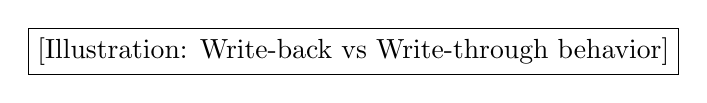
\begin{tikzpicture}[scale=0.7]
    % Placeholder for illustration
    \node[draw, rectangle] (note) {[Illustration: Write-back vs Write-through behavior]};
\end{tikzpicture}
\end{center}
\end{frame}

\begin{frame}{Review: Write Miss Policies}
\textbf{Write Allocate}
\begin{itemize}
    \item On miss, send request to lower level to fetch the block
    \item Before fetching block from lower level, free appropriate space (set and replacement policy)
\end{itemize}

\textbf{No Write Allocate}
\begin{itemize}
    \item On miss, send the write request itself to lower level
    \item No fetching of block to the required level
\end{itemize}

\begin{center}
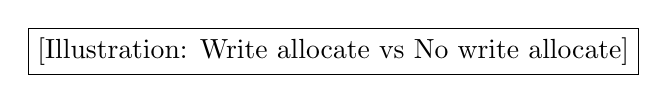
\begin{tikzpicture}[scale=0.7]
    % Placeholder for illustration
    \node[draw, rectangle] (note) {[Illustration: Write allocate vs No write allocate]};
\end{tikzpicture}
\end{center}
\end{frame}

\begin{frame}{The Inclusion Principle}
\begin{itemize}
    \item In a hierarchical cache working according to the inclusion principle, each level contains all the lines (not necessarily the most updated data - remember: WB/WT) that are in higher-level caches (closer to CPU)
    \item This is designed to simplify the communication protocols between levels
    \item The principle is not implemented in all processors
\end{itemize}

\begin{center}
\memoryhierarchy[0.8]
\end{center}
\end{frame}

\begin{frame}{Inclusion Principle - Eviction}
\textbf{Key Rule:} To maintain the inclusion principle:

\begin{itemize}
    \item When a cache line is evicted from a lower-level cache (L2 or L3)
    \item The same line must be evicted from all higher-level caches (closer to CPU)
    \item This ensures lower levels always contain data from upper levels
\end{itemize}

\vspace{0.3cm}
\begin{center}
\memoryhierarchy[0.8]
\end{center}
\end{frame}

\begin{frame}{Question 2: Cache Hierarchy Usefulness}
\textbf{Given:} A system with L2 cache where the inclusion principle is maintained.

\textbf{Question:} For each case below, is L2 useful?

\vspace{0.4cm}
\begin{columns}[T]
\begin{column}{0.35\textwidth}
\begin{enumerate}
\item Both cache levels are the same size
\begin{itemize}
    \small
    \item L1: direct mapped
    \item L2: fully associative
\end{itemize}
\end{enumerate}

\vspace{0.4cm}
\onslide<2->{
\textbf{Answer:} \textcolor{green!60!black}{\textbf{USEFUL}}

\small\textit{Reason:} L2's higher associativity prevents conflict misses.}
\end{column}

\begin{column}{0.65\textwidth}
\begin{center}
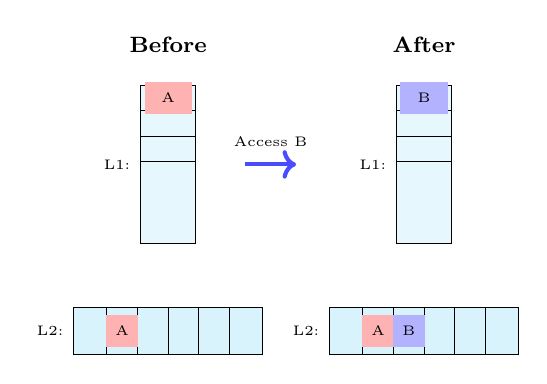
\begin{tikzpicture}[scale=0.65, node distance=0.4cm]
    % Define styles
    \tikzstyle{cacheA}=[fill=red!30]
    \tikzstyle{cacheB}=[fill=blue!30]

    % Left side - Before
    \node[above] at (0, 2) {\footnotesize\textbf{Before}};

    % L1 cache - left side (direct mapped with cells)
    \node[draw, rectangle, fill=cyan!10, minimum width=0.7cm, minimum height=2cm, label=left:{\tiny L1:}] (l1left) at (0,0) {};
    % Draw horizontal lines for direct-mapped cells (3 internal dividers for 4 cells)
    \foreach \y in {0.5, 1, 1.5} {
        \draw ([yshift=-\y cm]l1left.north west) -- ([yshift=-\y cm]l1left.north east);
    }
    \node[cacheA, minimum width=0.6cm, minimum height=0.4cm] at ([yshift=-0.25cm]l1left.north) {\tiny A};

    % L2 cache - left side (fully associative)
    \node[draw, rectangle, fill=cyan!15, minimum width=2.4cm, minimum height=0.6cm, below=0.8cm of l1left, label=left:{\tiny L2:}] (l2left) {};
    % Draw vertical lines for fully-associative cells using loop
    \foreach \x in {-1.2, -0.6, 0, 0.6, 1.2} {
        \draw ([xshift=\x cm]l2left.north) -- ([xshift=\x cm]l2left.south);
    }
    \node[cacheA, minimum width=0.4cm, minimum height=0.4cm] at ([xshift=-0.9cm]l2left.center) {\tiny A};

    % Arrow
    \draw[->, thick, blue!70, line width=1.5pt] (1.5,0) -- (2.5,0);
    \node[above] at (2, 0.15) {\tiny Access B};

    % Right side - After (moved further right)
    \node[above] at (5, 2) {\footnotesize\textbf{After}};

    % L1 cache - right side
    \node[draw, rectangle, fill=cyan!10, minimum width=0.7cm, minimum height=2cm, label=left:{\tiny L1:}] (l1right) at (5,0) {};
    % Draw horizontal lines for direct-mapped cells (3 internal dividers for 4 cells)
    \foreach \y in {0.5, 1, 1.5} {
        \draw ([yshift=-\y cm]l1right.north west) -- ([yshift=-\y cm]l1right.north east);
    }
    \node[cacheB, minimum width=0.6cm, minimum height=0.4cm] at ([yshift=-0.25cm]l1right.north) {\tiny B};

    % L2 cache - right side
    \node[draw, rectangle, fill=cyan!15, minimum width=2.4cm, minimum height=0.6cm, below=0.8cm of l1right, label=left:{\tiny L2:}] (l2right) {};
    % Draw vertical lines using loop
    \foreach \x in {-1.2, -0.6, 0, 0.6, 1.2} {
        \draw ([xshift=\x cm]l2right.north) -- ([xshift=\x cm]l2right.south);
    }
    \node[cacheA, minimum width=0.4cm, minimum height=0.4cm] at ([xshift=-0.9cm]l2right.center) {\tiny A};
    \node[cacheB, minimum width=0.4cm, minimum height=0.4cm] at ([xshift=-0.3cm]l2right.center) {\tiny B};
\end{tikzpicture}
\end{center}
\end{column}
\end{columns}
\end{frame}

\begin{frame}{Question 2: Continued}
\begin{enumerate}
\setcounter{enumi}{1}
\item Access time for both cache levels is identical. L2 is larger than L1.

\vspace{0.3cm}
\onslide<2->{
\textbf{Answer:} \textcolor{green!60!black}{\textbf{USEFUL}}

\textit{Reason:} L2 provides more capacity. However, L1 becomes less beneficial since both have the same access time.
}

\vspace{0.5cm}
\item<3-> Access time to L2 and main memory is identical.

\vspace{0.3cm}
\onslide<4->{
\textbf{Answer:} \textcolor{red!70!black}{\textbf{NOT USEFUL}}

\textit{Reason:} L2 offers no speed advantage over main memory, making it redundant.
}
\end{enumerate}
\end{frame}

\begin{frame}{Inclusion Principle - Snooping}
\textbf{Snoop:} Check higher-level caches when an entry is victimized to maintain inclusion

\begin{itemize}
    \item When a cache level wants to delete certain data, it checks higher-level caches (closer to CPU) to see if the data is also there
    \item If yes, it must be deleted first to maintain the inclusion principle
\end{itemize}

All caches work according to:
\begin{itemize}
    \item Write-back policy
    \item LRU replacement policy
    \item Maintain inclusion principle
\end{itemize}
\end{frame}

\begin{frame}{Inclusion Principle - Process Flow}
\small
Process from discovering need for line replacement in L3 until stabilization:

\begin{enumerate}
    \item L1 identifies read miss and requests data from L2
    \item L2 identifies read miss and requests data from L3
    \item L3 identifies read miss and selects line for replacement
    \item \textbf{Snoops:}
    \begin{itemize}
        \item L3 snoops to L2 to check if copy exists
        \item If copy in L2, L2 snoops to L1
        \item If copy in L1 is modified (M), write it to L2
        \item L1 marks line as invalid (I)
        \item If copy in L2 is modified (M), write it to L3
        \item L2 marks line as invalid (I)
    \end{itemize}
    \item If evicted line from L3 is in M state, write to main memory
    \item L3 reads required line from main memory and updates LRU
    \item Continue propagation to L2 and L1...
\end{enumerate}
\end{frame}

\begin{frame}{Inclusion Principle - Complete Flow Diagram}
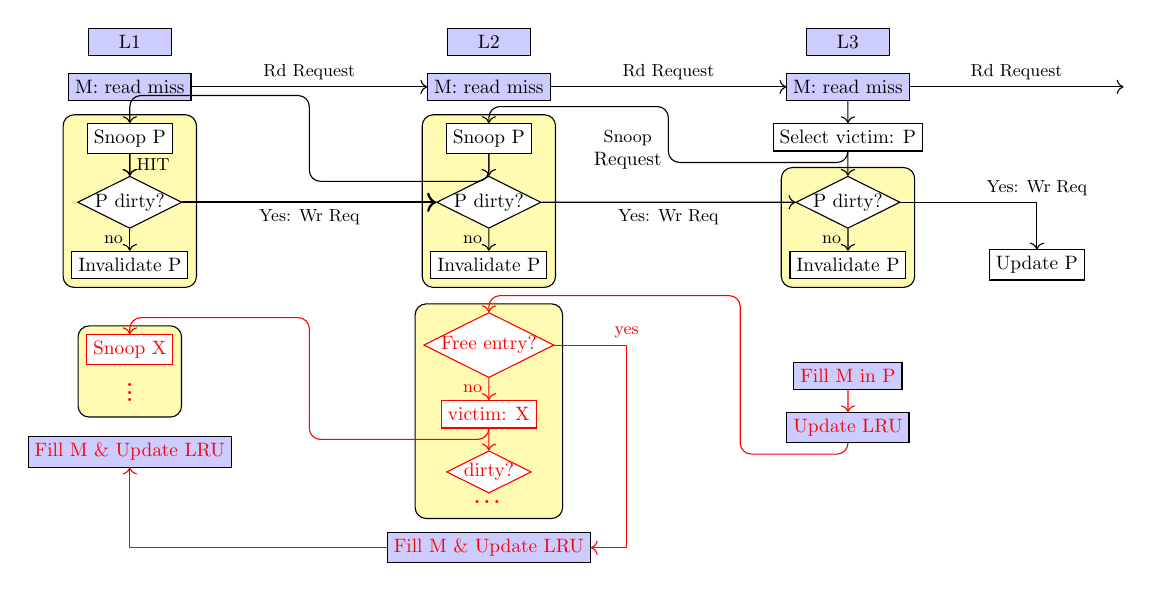
\begin{tikzpicture}[
    scale=0.7, transform shape,
    box/.style={rectangle, draw, minimum width=1.5cm, minimum height=0.5cm},
    decision/.style={diamond, draw, aspect=2, inner sep=0pt, minimum width=1cm, fill=white},
    reddecision/.style={decision, draw=red, text=red},
    bluebox/.style={box, fill=blue!20},
    yellowbox/.style={box, fill=yellow},
    whitebox/.style={box, fill=white},
    redbox/.style={box, fill=white, draw=red, text=red},
    bluered/.style={bluebox, text=red},
    yellowbg/.style={fill=yellow!30, draw=black, rounded corners, inner sep=3pt},
    every edge/.style={draw, ->, >=stealth},
    node distance=0.4cm and 1.5cm
]

% L1 Section
\node[bluebox] (l1) {L1};
\node[bluebox, below=0.3cm of l1] (l1read) {M: read miss};

\node[whitebox, below=of l1read] (snoopp1) {Snoop P};
\node[decision, below=of snoopp1] (dirty1) {P dirty?};
\node[whitebox, below=of dirty1] (inv1) {Invalidate P};
\node[redbox, below=1cm of inv1] (snoopx1) {Snoop X};
\node[below=0cm of snoopx1.south, text=red, anchor=north] (vdotsx1) {\textbf\vdots};

% L2 Section
\node[bluebox, right=5cm of l1] (l2) {L2};
\node[bluebox, below=0.3cm of l2] (l2read) {M: read miss};

\node[whitebox, below=of l2read] (snoopp2) {Snoop P};
\node[decision, below=of snoopp2] (dirty2) {P dirty?};
\node[whitebox, below=of dirty2] (inv2) {Invalidate P};

\node[reddecision, below=0.6cm of inv2] (free) {Free entry?};
\node[redbox, below=of free] (victimx) {victim: X};
\node[reddecision, below=of victimx] (dirtyx) {dirty?};
\node[below=0cm of dirtyx.south, text=red, anchor=north] (ldots2) {\textbf\ldots};

% L3 Section
\node[bluebox, right=5cm of l2] (l3) {L3};
\node[bluebox, below=0.3cm of l3] (l3read) {M: read miss};

\node[whitebox, below=of l3read] (select3) {Select victim: P};
\node[decision] at (select3 |- dirty2) (dirty3) {P dirty?};
\node[whitebox, below=of dirty3] (inv3) {Invalidate P};
\node[whitebox, right=of inv3] (update) {Update P};

\node[bluered, below=1.5cm of inv3] (fillm3) {Fill M in P};
\node[bluered, below=of fillm3] (updatelru) {Update LRU};
\node[bluered, below=of ldots2] (fillm2) {Fill M \& Update LRU};
\node[bluered, below=1.3cm of snoopx1] (fillm1) {Fill M \& Update LRU};

\begin{scope}[on background layer]
\node[yellowbg, fit=(snoopp1)(dirty1)(inv1)] {};
\node[yellowbg, fit=(snoopx1)(vdotsx1)] {};
\node[yellowbg, fit=(snoopp2)(dirty2)(inv2)] {};
\node[yellowbg, fit=(dirty3)(inv3)] {};
\node[yellowbg, fit=(free)(victimx)(dirtyx)(ldots2)] {};
\end{scope}

% Arrows with labels
\draw[->] (l1read) -- node[above, sloped] {\small Rd Request} (l2read);
\draw[->] (l2read) -- node[above, sloped] {\small Rd Request} (l3read);
\draw[->] (l3read) -- node[above, sloped] {\small Rd Request} ++(5,0);

\draw[->] (snoopp1) -- (dirty1);
\draw[->] (dirty1) -- node[left] {\small no} (inv1);
\draw[thick, ->] (dirty1.east) -- (dirty2.west) node[midway,below, align=center] {\small Yes: Wr Req};
\draw[->] (snoopp1) -- (dirty1) node[midway, right] {\small HIT};

\draw[->] (snoopp2) -- (dirty2);

% the routed path
\draw[->, rounded corners]
  (snoopp2.south)
  -- ++(0,-0.5)                               % down 0.5
  -| ($(snoopp1)!0.5!(snoopp2)$)                                  % over to midpoint x
  |- ($ (snoopp1.north) + (0,0.5) $)          % up to 0.5 above snoopp1.north
  -- (snoopp1.north);                         % straight down

\draw[->] (dirty2) -- node[left] {\small no} (inv2);

\draw[->](dirty2) -- node[below] {\small Yes: Wr Req} (dirty3.west);

\draw[->, red] (free) -| node[above] {\small yes} ++(2.5,0) |- (fillm2);
\draw[->, red] (free) -- node[left] {\small no} (victimx);
\draw[->, red] (victimx) -- (dirtyx);

\draw[->, red, rounded corners]
  (victimx.south)
  -- ++(0,-0.2)                               % down 0.5
  -| ($(victimx)!0.5!(snoopx1)$)                                  % over to midpoint x
  |- ($ (snoopx1.north) + (0,0.3) $)          % up to 0.5 above snoopp1.north
  -- (snoopx1.north);

\draw[->] (l3read) -- (select3);

\draw[->, rounded corners]
  (select3.south)
  -- ++(0,-0.2)                               % down 0.5
  -| ($(snoopp2)!0.5!(select3)$)                                  % over to midpoint x
  node[midway, left, near end, align=center] {\small Snoop\\Request}
  |- ($ (snoopp2.north) + (0,0.3) $)          % up to 0.5 above snoopp1.north
  -- (snoopp2.north);                         % straight down


\draw[->] (select3) -- (dirty3);
\draw[->] (dirty3) -- node[left] {\small no} (inv3);
\draw[->] (dirty3) -| node[above,midway] {\small Yes: Wr Req} (update);

% Bottom connections
\draw[->, red] (fillm3) -- (updatelru);
\draw[->, red, rounded corners]
  (updatelru.south)
  -- ++(0,-0.2)                               % down 0.5
  -| ($(updatelru)!0.3!(free)$)                                  % over to midpoint x
  |- ($ (free.north) + (0,0.3) $)          % up to 0.5 above snoopp1.north
  -- (free.north);                         % straight down                    % straight down

\draw[->, red] (fillm2) -| (fillm1);

\end{tikzpicture}
\end{frame}

\begin{frame}{Question 3: Write Miss Policy Deduction}
\textbf{Given:}
\begin{itemize}
    \item 3-level cache hierarchy with inclusion principle
    \item L2 and L3: \textbf{no write allocate} policy
    \item CPU writes to address \texttt{n} (causes L1 miss)
    \item This write causes an eviction from L3
\end{itemize}

\vspace{0.4cm}
\textbf{Question:} What is L1's write miss policy?

\vspace{0.4cm}
\onslide<2->{
\textbf{Answer:} \textcolor{blue!70!black}{\textbf{Write Allocate}}

\vspace{0.2cm}
\textit{Reasoning:} The L3 eviction proves that data was fetched into the cache hierarchy. With no-write-allocate at L2/L3, only L1's write-allocate policy could trigger this fetch.
}
\end{frame}

\begin{frame}{Question 4: Cache Configuration}
Given a processor with two cache levels:
\begin{itemize}
    \item Address size: 32 bits
    \item Cache line size for both caches: 32 bytes
    \item Write policy: Write-back for both
    \item Replacement policy: LRU for both
    \item Inclusion principle is maintained
    \item L1: 1KB, 2-way set associative
    \item L2: 4KB, 2-way set associative
\end{itemize}
\end{frame}

\begin{frame}[fragile]{Question 4: Program}
Consider the following program:

\begin{tcolorbox}[
    colback=blue!5,
    colframe=blue!40!black,
    boxrule=0.8pt,
    arc=3mm,
    left=3mm,
    right=3mm,
    top=2mm,
    bottom=2mm,
    fontupper=\footnotesize
]
\begin{lstlisting}[
    language=C,
    basicstyle=\ttfamily\scriptsize,
    keywordstyle=\color{blue!70!black}\bfseries,
    commentstyle=\color{green!50!black}\itshape,
    stringstyle=\color{orange},
    identifierstyle=\color{black},
    showstringspaces=false,
    numbers=left,
    numberstyle=\tiny\color{gray!70},
    stepnumber=1,
    numbersep=8pt,
    backgroundcolor=\color{white},
    breaklines=false,
    captionpos=b,
    keepspaces=true,
    morekeywords={int}
]
int arr[512];
int S = 0;
for (int i = 0; i < 2; i++) {
    for (int j = 0; j < 512; j++) {
        S += arr[j];
    }
}
\end{lstlisting}
\end{tcolorbox}

\vspace{0.3cm}
\textbf{Assumptions:}
\begin{itemize}
    \small
    \item Variables \texttt{i}, \texttt{j}, \texttt{S} and pointer \texttt{arr} are stored in registers
    \item Integer size is 4 bytes
    \item Cache is empty at program start
    \item Array is aligned in memory
\end{itemize}
\end{frame}

\begin{frame}{Question 4a: L1 Hit Rate}
\textbf{Analysis:}
\begin{itemize}
    \item We traverse the array twice
    \item In the first iteration of outer loop, we only miss when reading a new block
    \item Since cache line size is 32 bytes and integer size is 4 bytes, we fit 8 elements per block
    \item We only miss on 1 out of every 8 accesses
    \item Therefore, hit rate (HR) = $\frac{7}{8}$
\end{itemize}

For the second iteration:
\begin{itemize}
    \item At the start, cache will only contain the second half of array (elements 256--511) due to LRU policy
    \item We'll have misses for all first accesses to blocks containing elements 0--255
    \item Overall HR for entire program = $\frac{7}{8}$
\end{itemize}
\end{frame}

\begin{frame}{Question 4b: L2 Hit Rate}
\textbf{L2 Hit Rate} is defined as the percentage of memory access requests to L2 where a hit occurs (only considering requests where there was a miss in L1).

\begin{itemize}
    \item In first iteration, we only access cache on block transitions
    \item Since L2 is empty at start, first access always misses (HR = 0 for first iteration)
    \item L2 is large enough (4KB) to hold entire array
    \item In second iteration, every access to L2 will be a hit
    \item Overall L2 HR = $\frac{1}{2}$
\end{itemize}
\end{frame}

\begin{frame}{Question 4c: Adding L3 Cache}
Adding an L3 cache of 8MB size. L3 access time is about half of memory access time.

\textbf{Question:} How will adding L3 affect program performance (assuming it starts empty)?

\vspace{0.5cm}
\onslide<2->{
\textbf{Answer:}
\begin{itemize}
    \item The only misses in L2 are compulsory misses
    \item In L3, we'll still only have compulsory misses
    \item Therefore, no performance improvement
    \item However, misses in L2 are now more expensive (need additional L3 access before memory)
    \item Overall, performance will \textcolor{red!70!black}{\textbf{degrade}}
\end{itemize}
}
\end{frame}

\begin{frame}[fragile]{Question 5: Prefetching}
Program for calculating average grades:

\vspace{0.3cm}
\begin{tcolorbox}[
    colback=gray!5,
    colframe=gray!50,
    boxrule=0.5pt,
    arc=2mm,
    left=2mm,
    right=2mm,
    top=1mm,
    bottom=1mm,
    fontupper=\small
]
\begin{lstlisting}[
    language=C,
    basicstyle=\ttfamily\footnotesize,
    keywordstyle=\color{blue}\bfseries,
    commentstyle=\color{green!60!black},
    stringstyle=\color{orange},
    showstringspaces=false,
    numbers=left,
    numberstyle=\tiny\color{gray},
    stepnumber=1,
    numbersep=5pt,
    backgroundcolor=\color{white},
    breaklines=true,
    captionpos=b,
    keepspaces=true,
    escapeinside={(*@}{@*)},
    morekeywords={sum, average}
]
sum = 0;
for (i = 0; i < NUM_STUDENTS; i++) {
    sum += grades[i];
}
average = sum / NUM_STUDENTS;
\end{lstlisting}
\end{tcolorbox}

\vspace{0.2cm}
\begin{itemize}
    \item Each element in \texttt{grades} is 4 bytes
    \item L1 cache line size is 16 bytes
    \item Time to fetch a line from memory is 32 cycles
    \item Operation time with HIT in L1 is one clock cycle
\end{itemize}

Design a hardware prefetch system to improve L1 hit rate.
\end{frame}

\begin{frame}{Question 5: Solution}
\textbf{Prefetch System Design:}

\begin{itemize}
    \item An efficient prefetch system should issue a cache line fetch request with timing such that when the demand request arrives, the line is already in cache
    \item In our case, \textcolor{blue!70!black}{\textbf{32 clock cycles}} are needed to bring a line to cache
    \item Therefore, the prefetch system should be timed to generate a request \textcolor{blue!70!black}{\textbf{32 clock cycles before}} the program requests that address
\end{itemize}

\vspace{0.3cm}
\textbf{Prefetch Algorithm:}
\begin{itemize}
    \item Use a stride prefetch algorithm (detects sequential access pattern)
    \item Each cache line holds \textcolor{blue!70!black}{\textbf{4 array elements}} ($\frac{16 \text{ bytes}}{4 \text{ bytes}} = 4$ elements)
    \item Accessing 4 elements per line takes $4 \times 1 = 4$ cycles
    \item To cover the 32-cycle memory latency, we need to prefetch $\frac{32}{4} = 8$ lines ahead
    \item Therefore: On every access to line $n$, generate a prefetch request for line \textcolor{red!70!black}{\textbf{$n+8$}}
    \item This ensures data arrives in cache just in time when needed
\end{itemize}
\end{frame}

\begin{frame}{Question 5: Prefetch Timing Diagram}
\vspace{-0.2cm}
\begin{itemize}
    \item \textbf{Key insight:} Prefetch requests (yellow) are issued 32 cycles before data is needed
    \item When instructions 0-3 execute (cycles 32-35), data from Line0 is already valid (green)
\end{itemize}

\vspace{0.2cm}
\begin{center}
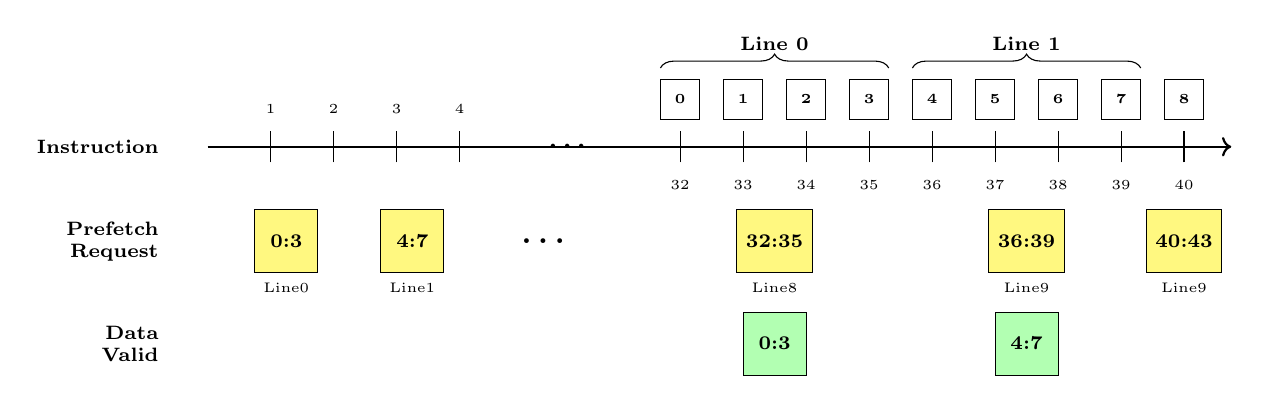
\begin{tikzpicture}[
    scale=1,
    instbox/.style={rectangle, draw, minimum height=0.5cm, minimum width=0.5cm, font=\tiny},
    cache/.style={rectangle, draw, fill=green!30, minimum height=0.8cm, minimum width=0.8cm, font=\scriptsize\bfseries},
    prefetch/.style={rectangle, draw, fill=yellow!50, minimum height=0.8cm, minimum width=0.8cm, font=\scriptsize\bfseries}
]
    % Timeline axis - shorter to fit inside figure
    \draw[->, thick] (0,0) -- (13,0);

    % Instruction label - aligned with instruction boxes
    \node[left, align=right, font=\scriptsize\bfseries] at (-0.5, 0) {Instruction};

    % Instruction tick marks (1-4, then ..., then cycles 32-40)
    \foreach \i in {1,2,3,4} {
        \node[above, font=\tiny] at (\i*0.8, 0.3) {\i};
        \draw (\i*0.8, -0.2) -- (\i*0.8, 0.2);
    }

    % Dots separator
    \node[font=\normalsize\bfseries] at (4.6, 0) {\dots};

    % Cycle numbers 32-40 with tick marks
    \foreach \i/\addr in {0/32, 1/33, 2/34, 3/35, 4/36, 5/37, 6/38, 7/39, 8/40} {
        \node[below, font=\tiny] at (6+\i*0.8, -0.3) {\addr};
        \draw (6+\i*0.8, -0.2) -- (6+\i*0.8, 0.2);
    }

    % Instruction boxes (0-8) positioned above the timeline, aligned with cycle numbers
    \node[instbox] at (6, 0.6) {\textbf{0}};
    \node[instbox] at (6.8, 0.6) {\textbf{1}};
    \node[instbox] at (7.6, 0.6) {\textbf{2}};
    \node[instbox] at (8.4, 0.6) {\textbf{3}};
    \node[instbox] at (9.2, 0.6) {\textbf{4}};
    \node[instbox] at (10, 0.6) {\textbf{5}};
    \node[instbox] at (10.8, 0.6) {\textbf{6}};
    \node[instbox] at (11.6, 0.6) {\textbf{7}};
    \node[instbox] at (12.4, 0.6) {\textbf{8}};

    % Line groupings with braces (not mirrored = upright) - above the instruction boxes
    \draw[decorate, decoration={brace, amplitude=5pt}] (5.75,1.0) -- (8.65,1.0);
    \node[above, font=\scriptsize\bfseries] at (7.2, 1.1) {Line 0};

    \draw[decorate, decoration={brace, amplitude=5pt}] (8.95,1.0) -- (11.85,1.0);
    \node[above, font=\scriptsize\bfseries] at (10.4, 1.1) {Line 1};

    % Prefetch Request row - closer to timeline
    \node[left, align=right, font=\scriptsize\bfseries] at (-0.5, -1.2) {Prefetch\\Request};
    \node[prefetch] (p1) at (1, -1.2) {0:3};
    \node[below, font=\tiny] at (p1.south) {Line0};

    \node[prefetch] (p2) at (2.6, -1.2) {4:7};
    \node[below, font=\tiny] at (p2.south) {Line1};

    \node[font=\large\bfseries] at (4.3, -1.2) {\dots};

    % Aligned to cycle 32 (x=6)
    \node[prefetch] (p3) at (7.2, -1.2) {32:35};
    \node[below, font=\tiny] at (p3.south) {Line8};

    % Aligned to cycle 36 (x=9.2)
    \node[prefetch] (p4) at (10.4, -1.2) {36:39};
    \node[below, font=\tiny] at (p4.south) {Line9};

    % Aligned to cycle 40 (x=12.4)
    \node[prefetch] (p5) at (12.4, -1.2) {40:43};
    \node[below, font=\tiny] at (p5.south) {Line9};

    % Data Valid row - closer to Prefetch Request
    \node[left, align=right, font=\scriptsize\bfseries] at (-0.5, -2.5) {Data\\Valid};
    \node[cache] at (7.2, -2.5) {0:3};
    \node[cache] at (10.4, -2.5) {4:7};

\end{tikzpicture}
\end{center}
\end{frame}

\end{document}